% This file was converted to LaTeX by Writer2LaTeX ver. 1.0.2
% see http://writer2latex.sourceforge.net for more info
\documentclass[a4paper]{article}
\usepackage[ascii]{inputenc}
\usepackage[T1]{fontenc}
\usepackage[spanish,dutch,english]{babel}
\usepackage{amsmath}
\usepackage{amssymb,amsfonts,textcomp}
\usepackage{color}
\usepackage{array}
\usepackage{supertabular}
\usepackage{hhline}
\usepackage{hyperref}
\hypersetup{pdftex, colorlinks=true, linkcolor=blue, citecolor=blue, filecolor=blue, urlcolor=blue, pdftitle=, pdfauthor=Ruben Perez Pascual, pdfsubject=, pdfkeywords=}
\usepackage[pdftex]{graphicx}
% Text styles
\newcommand\textstyleHyperlink[1]{\textcolor{blue}{#1}}
% Outline numbering
\setcounter{secnumdepth}{4}
\renewcommand\thesection{\arabic{section}}
\renewcommand\thesubsection{\arabic{section}.\arabic{subsection}}
\renewcommand\thesubsubsection{\arabic{section}.\arabic{subsection}.\arabic{subsubsection}}
\renewcommand\theparagraph{\arabic{section}.\arabic{subsection}.\arabic{subsubsection}.\arabic{paragraph}}
\makeatletter
\newcommand\arraybslash{\let\\\@arraycr}
\makeatother
% List styles
\newcounter{saveenum}
\newcommand\liststyleLFOxlix{%
\renewcommand\theenumi{\arabic{enumi}}
\renewcommand\theenumii{\alph{enumii}}
\renewcommand\theenumiii{\roman{enumiii}}
\renewcommand\theenumiv{\arabic{enumiv}}
\renewcommand\labelenumi{\theenumi.}
\renewcommand\labelenumii{\theenumii.}
\renewcommand\labelenumiii{\theenumiii.}
\renewcommand\labelenumiv{\theenumiv.}
}
\newcommand\liststyleLFOxxxvii{%
\renewcommand\labelitemi{[F0B7?]}
\renewcommand\labelitemii{o}
\renewcommand\labelitemiii{[F0A7?]}
\renewcommand\labelitemiv{[F0B7?]}
}
\newcommand\liststyleLFOxxxii{%
\renewcommand\theenumi{\alph{enumi}}
\renewcommand\theenumii{\alph{enumii}}
\renewcommand\theenumiii{\roman{enumiii}}
\renewcommand\theenumiv{\arabic{enumiv}}
\renewcommand\labelenumi{\theenumi)}
\renewcommand\labelenumii{\theenumii.}
\renewcommand\labelenumiii{\theenumiii.}
\renewcommand\labelenumiv{\theenumiv.}
}
\newcommand\liststyleLFOxxxv{%
\renewcommand\theenumi{\alph{enumi}}
\renewcommand\theenumii{\alph{enumii}}
\renewcommand\theenumiii{\roman{enumiii}}
\renewcommand\theenumiv{\arabic{enumiv}}
\renewcommand\labelenumi{\theenumi)}
\renewcommand\labelenumii{\theenumii.}
\renewcommand\labelenumiii{\theenumiii.}
\renewcommand\labelenumiv{\theenumiv.}
}
\newcommand\liststyleLFOxxxiii{%
\renewcommand\theenumi{\arabic{enumi}}
\renewcommand\theenumii{\alph{enumii}}
\renewcommand\theenumiii{\roman{enumiii}}
\renewcommand\theenumiv{\arabic{enumiv}}
\renewcommand\labelenumi{\theenumi.}
\renewcommand\labelenumii{\theenumii.}
\renewcommand\labelenumiii{\theenumiii.}
\renewcommand\labelenumiv{\theenumiv.}
}
\newcommand\liststyleLFOxxxvi{%
\renewcommand\labelitemi{{}-}
\renewcommand\labelitemii{o}
\renewcommand\labelitemiii{[F0A7?]}
\renewcommand\labelitemiv{[F0B7?]}
}
\newcommand\liststyleLFOx{%
\renewcommand\theenumi{\alph{enumi}}
\renewcommand\theenumii{\alph{enumii}}
\renewcommand\theenumiii{\roman{enumiii}}
\renewcommand\theenumiv{\arabic{enumiv}}
\renewcommand\labelenumi{\theenumi)}
\renewcommand\labelenumii{\theenumii.}
\renewcommand\labelenumiii{\theenumiii.}
\renewcommand\labelenumiv{\theenumiv.}
}
\newcommand\liststyleLFOxxxiv{%
\renewcommand\theenumi{\alph{enumi}}
\renewcommand\theenumii{\alph{enumii}}
\renewcommand\theenumiii{\roman{enumiii}}
\renewcommand\theenumiv{\arabic{enumiv}}
\renewcommand\labelenumi{\theenumi)}
\renewcommand\labelenumii{\theenumii.}
\renewcommand\labelenumiii{\theenumiii.}
\renewcommand\labelenumiv{\theenumiv.}
}
\newcommand\liststyleLFOxxxviii{%
\renewcommand\theenumi{\roman{enumi}}
\renewcommand\theenumii{\alph{enumii}}
\renewcommand\theenumiii{\roman{enumiii}}
\renewcommand\theenumiv{\arabic{enumiv}}
\renewcommand\labelenumi{\theenumi)}
\renewcommand\labelenumii{\theenumii.}
\renewcommand\labelenumiii{\theenumiii.}
\renewcommand\labelenumiv{\theenumiv.}
}
\newcommand\liststyleLFOxxxix{%
\renewcommand\labelitemi{[F0B7?]}
\renewcommand\labelitemii{[F0B7?]}
\renewcommand\labelitemiii{o}
\renewcommand\labelitemiv{[F0B7?]}
}
\newcommand\liststyleLFOxl{%
\renewcommand\theenumi{\arabic{enumi}}
\renewcommand\theenumii{\alph{enumii}}
\renewcommand\theenumiii{\roman{enumiii}}
\renewcommand\theenumiv{\arabic{enumiv}}
\renewcommand\labelenumi{\theenumi.}
\renewcommand\labelenumii{\theenumii.}
\renewcommand\labelenumiii{\theenumiii.}
\renewcommand\labelenumiv{\theenumiv.}
}
\newcommand\liststyleLFOxli{%
\renewcommand\labelitemi{[F0B7?]}
\renewcommand\labelitemii{o}
\renewcommand\labelitemiii{[F0A7?]}
\renewcommand\labelitemiv{[F0B7?]}
}
% Page layout (geometry)
\setlength\voffset{-1in}
\setlength\hoffset{-1in}
\setlength\topmargin{0.4923in}
\setlength\oddsidemargin{0.9847in}
\setlength\textheight{9.7238in}
\setlength\textwidth{6.2985992in}
\setlength\footskip{0.4923in}
\setlength\headheight{0.4923in}
\setlength\headsep{0cm}
% Footnote rule
\setlength{\skip\footins}{1.1777999mm}
\renewcommand\footnoterule{\vspace*{-0.007in}\setlength\leftskip{0pt}\setlength\rightskip{0pt plus 1fil}\noindent\textcolor{black}{\rule{0.33\columnwidth}{0.007in}}\vspace*{1mm}}
% Pages styles
\makeatletter
\newcommand\ps@MP{
  \renewcommand\@oddhead{FP7-ICT-318389/DEIMOS/REPORT/PU/GEO-Cloud-D10.2}
  \renewcommand\@evenhead{\@oddhead}
  \renewcommand\@oddfoot{}
  \renewcommand\@evenfoot{\@oddfoot}
  \renewcommand\thepage{\arabic{page}}
}
\makeatother
\pagestyle{MP}
\setlength\tabcolsep{1mm}
\renewcommand\arraystretch{1.3}
\title{}
\author{Ruben Perez Pascual}
\date{2014-07-04T11:27:00Z}
\begin{document}
\begin{flushleft}
\tablehead{}
\begin{supertabular}{llll}
\multicolumn{1}{c}{
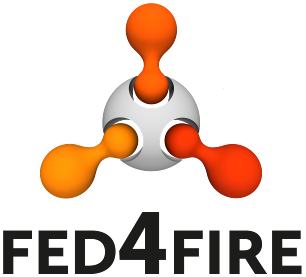
\includegraphics[width=1.43472in,height=1.30417in]{out-img1.png} } &
\multicolumn{1}{c}{
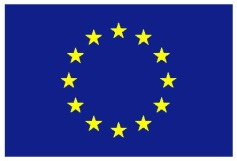
\includegraphics[width=1.07847in,height=0.73056in]{out-img2.jpg} } &
\multicolumn{1}{c}{

\includegraphics[width=1.27847in,height=0.88681in]{out-img3.jpg} } &
\multicolumn{1}{c}{

\includegraphics[width=1.30417in,height=1.06111in]{out-img4.png} }\\
\end{supertabular}
\end{flushleft}

\bigskip


\bigskip

\begin{flushleft}
\tablehead{}
\begin{supertabular}{|m{1.98856in}|m{4.25246in}|}
\hline
Project Acronym &
\bfseries Fed4FIRE\\\hline
Project Title &
\bfseries Federation for FIRE\\\hline
Instrument &
\bfseries Large scale integrating project (IP)\\\hline
Call identifier &
\bfseries FP7-ICT-2011-8\\\hline
Project number &
\bfseries 318389\\\hline
Project website &
\bfseries www.fed4fire.eu\\\hline
Experiment &
\bfseries GEO-Cloud\\\hline
\end{supertabular}
\end{flushleft}

\bigskip


\bigskip

{\centering\bfseries
Experiment problem statement and requirements\ report
\par}


\bigskip

\begin{flushleft}
\tablehead{}
\begin{supertabular}{|m{1.9649599in}|m{4.27466in}|}
\hline
Work\ package &
WP10\\\hline
Task &
T10.1.2\ GEO-Cloud Experiment\\\hline
Due date &
31/01/2014\\\hline
Submission date &
31/01/2014\\\hline
Report Lead &
F\'elix Pedrera\ (DEIMOS)\\\hline
Version &
1.0\\\hline
Authors &
\foreignlanguage{spanish}{F\'elix Pedrera}\foreignlanguage{spanish}{,
Gerardo Gonz\'alez, Jonathan
Becedas}\foreignlanguage{spanish}{\ }\foreignlanguage{spanish}{(DEIMOS)}\foreignlanguage{dutch}{\ }\\\hline
Reviewers &
Jonathan Becedas\ (DEIMOS)\\\hline
\end{supertabular}
\end{flushleft}

\bigskip


\bigskip

\begin{flushleft}
\tablehead{}
\begin{supertabular}{|m{1.9649599in}|m{4.27466in}|}
\hline
\bfseries Document ID &
\selectlanguage{spanish}\bfseries GEO-Cloud-D10.2\\\hline
Abstract &
In this document the experiment problem statement and the main
requirements that have to be fulfilled for its deployment in Fed4FIRE
are described.\\\hline
Keywords &
Deliverable\\\hline
\end{supertabular}
\end{flushleft}

\bigskip


\bigskip

\begin{flushleft}
\tablehead{}
\begin{supertabular}{m{1.9649599in}|m{0.31495985in}|m{3.36706in}|m{0.43505988in}|}
\hline
\multicolumn{1}{|m{1.9649599in}|}{Nature of the\ document} &
R &
Report &
X\\\hline
 &
P &
Prototype &
~
\\\hhline{~---}
 &
D &
Demonstrator &
~
\\\hhline{~---}
 &
O &
Other &
~
\\\hline
\multicolumn{1}{|m{1.9649599in}|}{Dissemination level} &
PU &
Public &
X\\\hline
 &
PP &
Restricted to other programme participants (including the Commission) &
~
\\\hhline{~---}
 &
RE &
Restricted to a group specified by the consortium (including
the\ Commission) &
~
\\\hhline{~---}
 &
CO &
Confidential, only for members of the consortium (including the
Commission) &
~
\\\hhline{~---}
\end{supertabular}
\end{flushleft}

\bigskip

\clearpage
\textrm{\textbf{Disclaimer}}


\bigskip

\textit{The information, documentation and figures available in this
deliverable, is written by the Fed4FIRE\ }(Federation for
FIRE)\ \textit{{}-- project consortium under EC co-financing contract
FP7-ICT-}\textit{318389}\textit{\ and does not necessarily reflect the
views of the European Commission}\textit{. The European
C}\textit{ommission is not liable for any use that may be made of the
information contained herein.}

\clearpage
\textrm{\textbf{Executive S}}\textrm{\textbf{ummary}}


\bigskip


\bigskip

In this deliverable the GEO-Cloud experiment is described. GEO-Cloud
will be deployed in the Fed4FIRE infrastructure. The works of design,
implementation, execution and validation of the experiment and final
reporting will be carried out by Elecnor Deimos.


\bigskip

This deliverable is based in the Description of Work of the experiment
together with the specifications of the Fed4FIRE infrastructures.


\bigskip

GEO-Cloud is a close to reality industry driven experiment that will go
beyond conventional services and infrastructures in the EO sector to
implement and test in cloud a complete EO system (from the acquisition
of geo-data with a constellation of satellites to its distribution to
end users with remote access). The main objective is to value if the
use of future internet technologies provides socio-economical viable
solutions applicable to industry to offer highly demanding services
such as crisis management in the EO sector.


\bigskip

The scenario is that of a constellation of satellites in Low Earth
Orbits that covers\ the Earth{\textquoteright}s surface in a daily
basis, the geo-data is downloaded in several ground stations
distributed around the world and transferred to the cloud for its
treatment and distribution. \ We will focus in two main use cases: i)
to offer basic satellite imagery services ii) to offer high added value
services with real time response to manage crisis events such as
natural disasters.\ 


\bigskip

GEO-Cloud will emulate the remote sensing mission with the satellites,
the topology network and the communications in the\ Virtual
Wall\ testbed. The data acquired from the emulated satellites will be
transferred to the\ BonFIRE\ cloud\ for storage,\ processing
and\ distribution of data.\ End users accessing and broadcasting will
be emulated in another network implemented in\ Virtual Wall. In order
to implement realistic impairments in Virtual Wall, real networks will
be tested in\ PlanetLab Europe. \ The technologies for imagery
distribution and EO service delivery using cloud technologies and
Internet protocols will be tested.


\bigskip

The document is divided into the following\ 8\ sections:\ Section 1 is
devoted to the introduction of the document, in Section 2 the
objectives of the experiment are described, Section 3 describes the
experiment, in Section 4 the experiment is designed, in Section 5 the
schedule of the experiment is exposed, Section 6 describes the ethical
issues, Section 7 shows the main conclusions and Section 8\ the
references cited throughout the text.

\clearpage
\textrm{\textbf{A}}\textrm{\textbf{cronyms and
A}}\textrm{\textbf{bbreviations}}


\bigskip

\begin{flushleft}
\tablehead{}
\begin{supertabular}{|m{0.8823598in}|m{5.35596in}|}
\hline
BF &
BonFIRE\\\hline
GS &
Ground Station\\\hline
Sat &
Satellite\\\hline
VM &
Virtual Machine\\\hline
VW &
Virtual Wall\\\hline
PLE &
PlanetLab Europe\\\hline
EO &
Earth Observation\\\hline
\end{supertabular}
\end{flushleft}
\clearpage
\textrm{\textbf{Table of C}}\textrm{\textbf{ontents}}


\bigskip

\setcounter{tocdepth}{3}
\tableofcontents

\bigskip

\section[Introduction]{Introduction}
\hypertarget{Toc378868684}{}
\bigskip

In this deliverable the GEO-Cloud experiment is described so as to the
plan for its implementation, execution and validation. The GEO-Cloud
experiment is one of the experiments that will be tested in the First
Open Call of Fed4FIRE:\ 1st Fed4FIRE Competitive Call for Additional
Project Partners.\ 


\bigskip

The description of Fed4FIRE can be found in the project
webpage\ \href{http://www.fed4fire.eu/home/project-info.html}{\textstyleHyperlink{http://www.fed4fire.eu}}.
It is as follows: {\textquotedblleft}\textit{Fed4FIRE is an Integrating
Project under the European Union{\textquoteright}s Seventh Framework
Programme (FP7) addressing the work programme topic Future
Intern}\textit{et Research and
Experimentation}{\textquotedblright}.\ The project is coordinated by
iMinds and will run for 48 months until September 2016.


\bigskip

The GEO-Cloud experiment main objective is to provide response to one of
the main challenges in the Earth Observation field: how to treat and
distribute massive amounts of data recorded by optical
satellites.\ Thus, the question to solve with the experiment is the
following:\ \textit{does cloud computing and}\textit{, in
general,}\textit{\ future internet
technolog}\textit{y}\textit{\ provide socio-economical viable solutions
for highly demanding services in Earth Observation?}\textit{\ }\ This
field\ is considered\ a key element in the European Research Road Map
and an opportunity market\ for the next years.\ Nevertheless, EO still
presents critical challenges that have to be overcome to cover the
demand of services that are currently offered but also to advance new
ones.\ 


\bigskip

EO industries implement on-site conventional infrastructures to acquire,
store, process and distribute the geo-information generated with the
recorded data. However these solutions have the risks of over/under
size the infrastructure, they are not flexible to cover sudden changes
in the demand of services and the access to the information presents
large latencies. These aspects limit the use of EO technology for real
time use such as to manage crises, natural disasters and civil security
among others\ (Deren, 2007).


\bigskip

The use of cloud computing technology can overcome the previously
defined limitations that present conventional infrastructures because
of its elasticity, scalability and on-demand use
characteristics\ (Armbrust, 2010).\ 


\bigskip

GEO-Cloud Experiment goes beyond conventional data infrastructures used
in EO industry and beyond the implementations of applications running
in cloud, to quest which parts of a complete infrastructure of EO are
technologically and economically viable to be virtualized to offer
basic and high added value services\ Figure 1.\ 


\bigskip

GEO-Cloud is implemented in three Fed4FIRE testbeds: PlanetLab Europe,
Virtual Wall and BonFIRE.

{\centering 
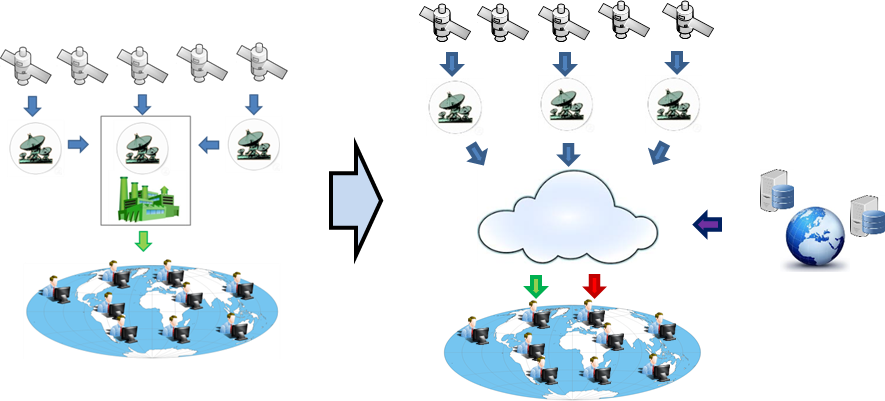
\includegraphics[width=2.4913in,height=2.06949in]{out-img5.png} \par}

{\bfseries
\label{bkm:Ref361933632}Figure\ 1\ The\ GEO-Cloud Concept.\ It is based
on the\ use\ of\ cloud technology to acquire data, store it, process
it, integrate it with other sources and distribute it to end
users\ with the final objective of\ testing\ viable solutions for its
real implementation.}

\section[GEO{}-Cloud Objectives]{GEO-Cloud Objectives}
\hypertarget{Toc378868685}{}
\bigskip

The experiment objectives are summarized as follows:


\bigskip

\liststyleLFOxlix
\setcounter{saveenum}{\value{enumi}}
\begin{enumerate}
\setcounter{enumi}{\value{saveenum}}
\item To implement in Fed4FIRE a close to real world Earth Observation
system.
\end{enumerate}

\bigskip

\liststyleLFOxlix
\setcounter{saveenum}{\value{enumi}}
\begin{enumerate}
\setcounter{enumi}{\value{saveenum}}
\item To test and validate the following models:
\end{enumerate}
\liststyleLFOxxxvii
\begin{itemize}
\item A global remote sensing model
\item A cloud model for Earth Observation
\item A model of end-users demand\ 
\end{itemize}

\bigskip

\liststyleLFOxlix
\setcounter{saveenum}{\value{enumi}}
\begin{enumerate}
\setcounter{enumi}{\value{saveenum}}
\item To compare the different types of services offered (basic and
added value services) to cover different types of demand.\ 
\end{enumerate}

\bigskip

\liststyleLFOxlix
\setcounter{saveenum}{\value{enumi}}
\begin{enumerate}
\setcounter{enumi}{\value{saveenum}}
\item To validate if future internet cloud computing and networks
provide viable solutions for conventional Earth Observation systems to
establish the basis for the implementation of EO infrastructures in
cloud.\ 
\end{enumerate}

\bigskip

\liststyleLFOxlix
\setcounter{saveenum}{\value{enumi}}
\begin{enumerate}
\setcounter{enumi}{\value{saveenum}}
\item To verify if the Fed4FIRE infrastructure and tools are appropriate
for running this complex, close to reality experiments.
\end{enumerate}

\bigskip

\section[Experiment Description]{Experiment Description}
\hypertarget{Toc378868686}{}
\bigskip

The experiment consists of virtualizing a conventional EO system to
offer on demand services to clients with the objective of validating
its viability, find the strengths and weaknesses of using cloud
computing technology and establish possible solutions for a future
implementation in the market. There are three components:

\liststyleLFOxxxii
\setcounter{saveenum}{\value{enumi}}
\begin{enumerate}
\setcounter{enumi}{\value{saveenum}}
\item \textbf{In-orbit mission:}\ this component generates the raw data.
This consists of un-processed images of the Earth captured by a
constellation of satellites and downloaded to different ground
stations.\ 
\item \textbf{Treatment of data:}\ the data has to be stored, processed
at different levels based on the services offered and distributed to
the clients. The data acquired by the in-orbit mission is integrated
with other sources to provide higher quality services.
\item \textbf{End-users:}\ users of the provided services with
different\ levels of remote access rights.\ 
\end{enumerate}
The system will be emulated at all levels for its monitoring and
control. In orbit mission and end-users traffic, accesses, network
topology, communications and data transfer will be emulated in Virtual
Wall and PlanetLab Europe. The tools, models and architecture to treat
the data will be implemented in the BonFIRE Cloud. Different parameters
will be controlled (bandwidth, latencies and other impairments) to
emulate a realistic system with different levels of demand.\ 


\bigskip

\paragraph{Scenario}
A constellation of\ 17\ satellites covers the surface of the Earth in
images in a daily basis.\ 


\bigskip

{\centering 
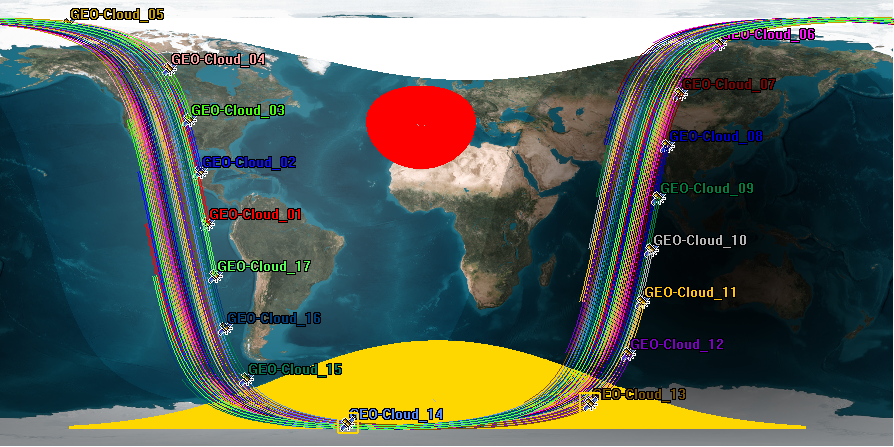
\includegraphics[width=2.59145in,height=2.14443in]{out-img6.png} \par}

{\centering\bfseries
Figure\ 2\ Ground tracks\ of the 17 GEO-Cloud satellites
\par}


\bigskip

The images are downloaded in real time to\ 12\ ground stations\ depicted
in\ Table 1.


\bigskip

{\centering\bfseries
\label{bkm:Ref377044034}Table\ 1\ Ground stations design, number of
accesses per day and duration of the passes
\par}

\begin{center}
\tablehead{\hline
\bfseries\color{black} Ground Station &
\bfseries\color{black} Accesses per day &
\bfseries\color{black} Accumulated duration (h)\\\hline}
\begin{supertabular}{m{0.98095983in}m{0.6288598in}m{0.90525985in}}
\bfseries\color{black} Irkutsk &
\raggedleft \color{black} 7 &
\raggedleft\arraybslash \color{black} 0.95\\
\bfseries\color{black} Puertollano &
\raggedleft \color{black} 4 &
\raggedleft\arraybslash \color{black} 0.62\\
\bfseries\color{black} Svalbard &
\raggedleft \color{black} 15 &
\raggedleft\arraybslash \color{black} 2.21\\
\bfseries\color{black} Troll &
\raggedleft \color{black} 11 &
\raggedleft\arraybslash \color{black} 1.69\\
\bfseries\color{black} Chetumal &
\raggedleft \color{black} 3 &
\raggedleft\arraybslash \color{black} 0.50\\
\bfseries\color{black} Cordoba &
\raggedleft \color{black} 4 &
\raggedleft\arraybslash \color{black} 0.53\\
\bfseries\color{black} Dubai &
\raggedleft \color{black} 4 &
\raggedleft\arraybslash \color{black} 0.57\\
\bfseries\color{black} Kourou &
\raggedleft \color{black} 4 &
\raggedleft\arraybslash \color{black} 0.49\\
\bfseries\color{black} Krugersdorp &
\raggedleft \color{black} 4 &
\raggedleft\arraybslash \color{black} 0.54\\
\bfseries\color{black} Malaysia &
\raggedleft \color{black} 3 &
\raggedleft\arraybslash \color{black} 0.42\\
\bfseries\color{black} Prince Albert &
\raggedleft \color{black} 6 &
\raggedleft\arraybslash \color{black} 0.93\\
\bfseries\color{black} Sidney &
\raggedleft \color{black} 4 &
\raggedleft\arraybslash \color{black} 0.61\\\hline
\bfseries\color{black} TOTAL &
\raggedleft \bfseries\color{black} 69 &
\raggedleft\arraybslash \bfseries\color{black} 10.07\\\hline
\end{supertabular}
\end{center}

\bigskip

The raw data is transferred from the ground stations to a cloud
computing infrastructure where the data is stored, processed on demand
at different levels and integrated with information obtained from
external sources to the system: sensors and other databases. \ All that
data is processed to generate geo-information which is distributed to
end-users to cover different levels of demand.\ 


\bigskip

There will be different types of demand\ of services\ for both basic
satellite imagery services and high added value services:\ constant
demand, variable demand and highly variable demand.\ The demand can
also have different types of loads associated, attending to three
components:\ processing load, storage load and communications load.
Possible combinations of them can also be presented. Types of load in
the demand:

\liststyleLFOxxxv
\setcounter{saveenum}{\value{enumi}}
\begin{enumerate}
\setcounter{enumi}{\value{saveenum}}
\item \textbf{Processing:}\ Different load levels for processing such as
minimum load, medium load and high load.
\item \textbf{Storage:}\ Different load levels for storage such as
minimum load, medium load and high load.
\item \textbf{Urgency}\textbf{:}\ Urgent responses with real time
requirement and not urgent responses without real time requirement.
\end{enumerate}
GEO-Cloud provides three types of services to the end-users. In those
types of services, representative use cases will be implemented for
testing:

\liststyleLFOxxxiii
\setcounter{saveenum}{\value{enumi}}
\begin{enumerate}
\setcounter{enumi}{\value{saveenum}}
\item \textbf{Basic satellite imagery services:}\ It includes accessing
to low and automated processed satellite images from catalog.\ The
basic service is a pull service, since the end users have to access the
cloud servers and retrieve the data.

\setcounter{saveenum}{\value{enumii}}
\begin{enumerate}
\setcounter{enumii}{\value{saveenum}}
\item Basic images: orthorectified images, images with\ minimum
geolocation.
\end{enumerate}
\end{enumerate}

\bigskip

To carry out the experiment we will use images from our catalog, and
public images from sources such as GMES,\ but we will not integrate
them in this\ service (just for testing). We will test the transfer of
data and accessing to the information in cloud with different loads of
processing. This will be used as a control for comparing with the rest
of services. We will test processing loads and timing to measure the
response of the system.


\bigskip

\liststyleLFOxxxiii
\setcounter{saveenum}{\value{enumi}}
\begin{enumerate}
\setcounter{enumi}{\value{saveenum}}
\item \textbf{High added value services:}\ \ It includes instant
accessing to automatically processed satellite images and data. In
this\ case, data from other sources will be used and integrated with
satellite imagery\ to combine the information and provide the service.
Online processing will be tested with different computing loads and
demands.\ Among the services that we will test we will focus in\ the
following:

\setcounter{saveenum}{\value{enumii}}
\begin{enumerate}
\setcounter{enumii}{\value{saveenum}}
\item \textbf{Pull type service:}\ Service under request.\ For example
the emulation of\ crisis management of natural catastrophes such
as\ the Lorca earthquake in
Spain\ (http://en.wikipedia.org/wiki/2011\_Lorca\_earthquake).\ 
\item \textbf{Push type service:}\ The system periodically and
automatically provides information to the end user without request.
Tracking of specific areas or mobiles, for example the tracking
of\ infrastructures\ in construction.\ More information about pull and
push strategies can be found in\ (Simchi-Levi, Kaminsky, \&
Simchi-Levy, 1999).
\end{enumerate}
\end{enumerate}

\bigskip

\liststyleLFOxxxiii
\setcounter{saveenum}{\value{enumi}}
\begin{enumerate}
\setcounter{enumi}{\value{saveenum}}
\item \textbf{Hosting}\textbf{\ services}\textbf{:}\ GEO-Cloud hosting
services will reserve space and access for the end-users to offer the
possibility of storing their own geo-data, which can have been
generated in the previous services. This solution is designed for
those\ users\ that do not foresee to acquire specific storage hardware
or do not want to invest on very large storage facilities.
\end{enumerate}
The end users{\textquoteright} load will be defined by attending the
following classification:


\bigskip

\liststyleLFOxxxvii
\begin{itemize}
\item Service Type:
\end{itemize}
\liststyleLFOxxxvi
\begin{itemize}
\item Basic

\begin{itemize}
\item Basic
\item Advanced
\end{itemize}
\item High added value:

\begin{itemize}
\item Pull\ 
\item Push
\end{itemize}
\item Hosting
\end{itemize}

\bigskip

\liststyleLFOxxxvii
\begin{itemize}
\item Loads in cloud technology:
\end{itemize}
\liststyleLFOxxxvi
\begin{itemize}
\item Processing

\begin{itemize}
\item Low
\item Medium
\item High
\end{itemize}
\item Storage

\begin{itemize}
\item Low\ 
\item Medium
\item High
\end{itemize}
\item Urgency

\begin{itemize}
\item Urgent
\item Not Urgent
\end{itemize}
\end{itemize}
\liststyleLFOxxxvii
\begin{itemize}
\item Demand Variability
\end{itemize}
\liststyleLFOxxxvi
\begin{itemize}
\item Constant
\item Variable
\item Highly Variable
\end{itemize}

\bigskip

The classification will allow us to analyse the technological and
economic viability of the services for their implementation in real
life. It will also allow us to find the limitations of the cloud
technology and establish requirements for its implementation.


\bigskip

\section[Experiment Design]{Experiment Design}
\hypertarget{Toc378868687}{}
\bigskip

\subsection[Implementation]{Implementation}
\hypertarget{Toc378868688}{}The GEO-Cloud experiment\ requires emulating
a complete realistic Earth Observation Mission to provide high added
value services such as crisis managemen.\ To this complex situation,
the system has to response by processing on demand massive and variable
amounts of stored and on line transferred data.


\bigskip

GEO-Cloud makes use of the following Fed4FIRE facilities: PlanetLab
Europe, Virtual Wall and BonFIRE. PlanetLab Europe allows us to measure
real network characteristics geographically distributed to setup our
models. Virtual Wall allows us to create any desired network topology
and emulate the in-orbit mission and the web service to the users.
BonFIRE provides us a real cloud infrastructure with observability in
all the layers to test our cloud based\ services.


\bigskip

\textbf{A.\ }\textbf{Implementation of the c}\textbf{loud based
service}\textbf{s in BonFIRE}\ 

To facilitate offering the previous services we propose to implement a
multi-layered cloud model in the\ BonFIRE\ cloud infrastructure to
generate on demand geo-information.\ The multi-layered cloud model is
constituted of two layers:


\bigskip

\liststyleLFOx
\setcounter{saveenum}{\value{enumi}}
\begin{enumerate}
\setcounter{enumi}{\value{saveenum}}
\item \textbf{Layer 1}\textbf{:\ }This layer involves the basic
satellite imagery services. \ It acquires the raw data, stores it, has
the first level of processing, distributes the processed data and
offers the hosting service.\ 
\item \textbf{Layer 2:\ }This layer involves the high added value
services.\ It can use historical processed,\ real time captured and
pre-processed data from layer 1. This layer processes the information
for real time generation of geo-information and offers real time access
and distribution to the end-users. Typically, the implementation of
high added value EO services involves\ the ingestion of the raster
imagery from the satellites into a spatial database or storage, where
it can be refined, simplified, processed or combined with other data
sources in vector or raster format. The products, which can be vector
or raster data, are distributed or queried using Internet technologies
(OGC standards like WMS) or through\ Web services\ (tiles, caches,
etcetera).\ 
\end{enumerate}
\textbf{B.\ }\textbf{Implementation of the a}\textbf{ccess to the
services}\textbf{\ in Virtual Wall and PlanetLab Europe}\ 

The access to the services will be done with different levels of
subscription. Thus, we can emulate that end-users can access the type
of information they really need, and we can analyse the demand of the
services we are offering. The access will be remote and will emulate a
web service. A\ Virtual Wall\ network will emulate end-users accessing
to the services.


\bigskip

Through the implementation of a network in PlanetLab Europe we will
measure the characteristics of the real network when end users around
the world remotely access the data: bandwidth, latencies, loss rate and
background noise.\ This information will be used to upload the
implemented model in Virtual Wall.\ 


\bigskip

With the Virtual Wall emulation we can have complete control of the
resources, compute the demand and all the factors involved in the
situation to test the system and record its behaviour under the
different conditions.


\bigskip

\textbf{C.\ }\textbf{Implementation of the a}\textbf{cquisition of
geo-data}\textbf{\ in Virtual Wall and PlanetLab Europe.}\ 

The acquisition of geo-data will be obtained from the in-orbit mission
and from external sources:\ 

\liststyleLFOxxxiv
\setcounter{saveenum}{\value{enumi}}
\begin{enumerate}
\setcounter{enumi}{\value{saveenum}}
\item \textbf{In-orbit mission:\ }The constellation of satellites and
the ground stations will be emulated in Virtual Wall. We will implement
a network topology to communicate the different satellites with the
ground stations. Every satellite in its orbit and every ground station
models will be simulated in a node.\ 
\end{enumerate}

\bigskip

The satellite models will simulate the orbits and the pass of the
satellites over the ground stations. The ground stations models will
simulate the coverture of the antennas and the download of the data.
When a satellite is inside this radius, the satellite downloads the
data to the ground station that is visible. The downloaded data in the
ground stations is transferred to the BonFIRE cloud.\ 


\bigskip

With the Virtual Wall network we will\ control bandwidths, latencies,
loss rates and background noise.\ We will also create a realistic
network topology to transfer data between different nodes.\ 


\bigskip

In order to determine the correct link characteristics for the
connections between the ground and the cloud infrastructure we will
measure appropriate values for the link impairment by measuring
the\ current\ characteristics between these different geographical
locations using the\ PlanetLab Europe\ testbed.\ 


\bigskip

\liststyleLFOxxxiv
\setcounter{saveenum}{\value{enumi}}
\begin{enumerate}
\setcounter{enumi}{\value{saveenum}}
\item \textbf{External sources:\ }We will acquire information from other
geo-data sources\ such as\ GMES\ database. That information will be
directly transferred to the BonFIRE cloud for its\ use.\ 
\end{enumerate}

\bigskip

If available, we will have preference for integrating information that
can be accessed programmatically through Web Services or APIs and with
an adequate reuse license, since it allows using and requesting only
the data needed by the service and reduces the needs of permanent
storage. This also serves as a use case to test how the integration
with other data providers and infrastructures affects the performance
of the services under the Geo-Cloud scenarios.\ 


\bigskip

Thus, the whole EO system will be completely implemented in Fed4FIRE,
see\ Figure 3.\ 

{\centering 
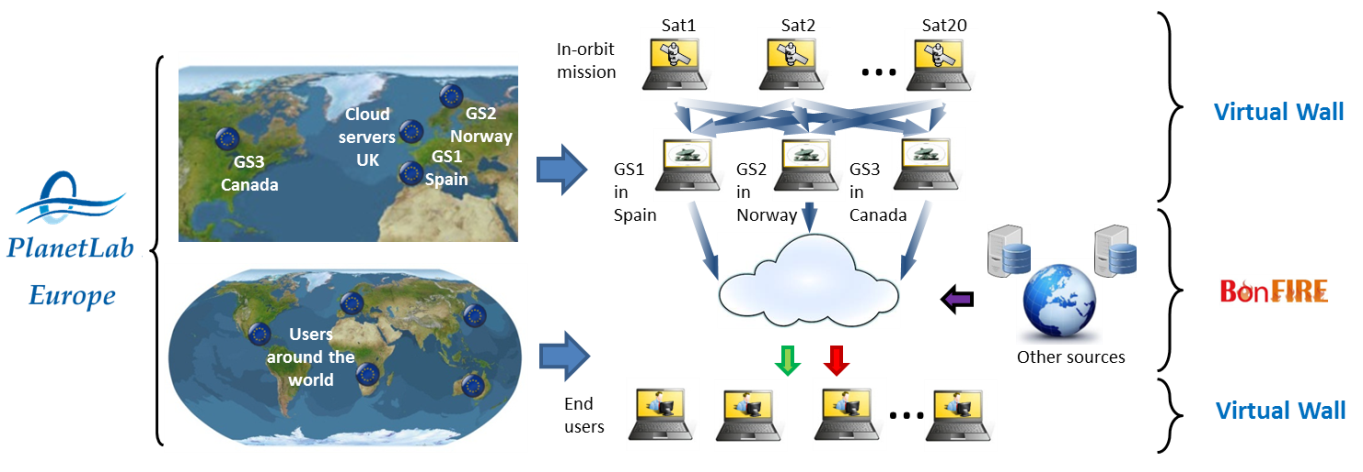
\includegraphics[width=6.18413in,height=2.15025in]{out-img7.png} \par}

{\centering\bfseries
\label{bkm:Ref361386330}Figure\ 3\ GEO-Cloud\ implementation\ in
Fed4FIRE
\par}


\bigskip

\subsection[Procedure]{Procedure}
\hypertarget{Toc378868689}{}
\bigskip

The experiment deployment includes the computation of image processing
algorithms and transfer of data from different nodes in an ad-hoc
created topology network that emulates a real Earth Observation System.


\bigskip

The experiment starts with\ the\ preparation of the\ software and
models\ that will be implemented\ in Fed4FIRE.\ Later\ we will start
implementing the different models in\ VW, BF\ and PLE.\ 


\bigskip

After the whole system is integrated in the Fed4FIRE testbeds the
experiment starts its execution and validation. This stage is separated
into two phases:\ 


\bigskip

\liststyleLFOxxxviii
\setcounter{saveenum}{\value{enumi}}
\begin{enumerate}
\setcounter{enumi}{\value{saveenum}}
\item Set of trials in PlanetLab Europe to\ monitor and test\ the link
characteristics between the different geographical distributed points:
virtual ground stations (GSs), cloud infrastructure and end users.\ 
\item Update\ of the models implemented in Virtual Wall with the
parameters measured in PlanetLab Europe.
\item Set of trials in the updated EO virtualized system implemented in
Virtual Wall and BonFIRE.\ To monitor the behavior of the system
implemented in the testbeds.
\end{enumerate}

\bigskip

\subsection[Parameters]{Parameters}
\label{bkm:Ref378661331}\hypertarget{Toc378868690}{}
\bigskip

The following parameters will be used as control and variables:


\bigskip

In\ the\ PlanetLab Europe\ tests:

\liststyleLFOxxxvii
\begin{itemize}
\item Control:\ 

\begin{itemize}
\item Bandwidth
\end{itemize}
\item Variables:\ 

\begin{itemize}
\item Latencies
\item Loss rate
\item Background noise
\end{itemize}
\end{itemize}

\bigskip

In\ the integrated system in\ Virtual Wall\ and BonFIRE:


\bigskip

\liststyleLFOxxxix
\begin{itemize}
\item Control:

\begin{itemize}
\item \begin{itemize}
\item Bandwidth
\item Loss rate
\item Background noise
\item Latencies
\end{itemize}
\item Variables:

\begin{itemize}
\item Processing time
\item Latency from image capture to distribution
\item Storage load
\item Processing load
\item Processing and storage strategy viability
\item Cues management
\item Performance of the system
\end{itemize}
\end{itemize}
\end{itemize}
\subsection[Requirements]{Requirements}
\hypertarget{Toc378868691}{}
\bigskip

The GEO-Cloud system was designed taking into account the following
requirements:


\bigskip

\textbf{REQ\_SYS\_0001:}\ The geo-information\ generated\ by the
satellites shall be in a daily basis.


\bigskip

\textbf{REQ\_SYS\_0002:}\ For the design of the satellite constellation,
a map of the Earth surface has to be daily\ generated.


\bigskip

\textbf{REQ\_SYS\_0003:}\ The geo-information has to be on demand
processed and distributed.


\bigskip

\textbf{REQ\_SYS\_0004:}\ The raw data acquisition from the satellites
follows an almost constant pattern.\ 


\bigskip

\textbf{REQ\_SYS\_0005:}\ The data acquired has to be stored and be
accessible to provide historical records.


\bigskip

The following requirements are those that the Fed4FIRE testbeds shall
fulfill for a correct implementation and execution of the experiment:


\bigskip

\textbf{REQ\_F4F\_0001:}\ The Fed4FIRE testbeds used in the GEO-Cloud
experiment shall allow the monitoring and control of the parameters
described in section\ 4.3.


\bigskip

\textbf{REQ\_F4F\_0002:}\ The Fed4FIRE testbeds\ shall allow transfer of
data with size\ in the order of GB\ between nodes.


\bigskip

\textbf{REQ\_F4F\_0003:}\ Fed4FIRE shall guarantee connectivity between
BonFIRE and Virtual Wall testbeds.


\bigskip

\textbf{REQ\_F4F\_00}\textbf{0}\textbf{4:}\ PlanetLab Europe shall
facilitate the use of\ at least 7\ nodes of PlanetLab Central.


\bigskip

\textbf{REQ\_F4F\_0005:}\ Virtual Wall shall provide at least 30 nodes
for the deployment of the GEO-Cloud experiment.


\bigskip

\textbf{REQ\_F4F\_00}\textbf{0}\textbf{6:}\ BonFIRE shall allow us to
script our own software in the cloud.


\bigskip

\textbf{REQ\_F4F\_0007:}\ Fed4FIRE shall guarantee the availability of
the testbeds used in the GEO-Cloud experiment for its implementation
and execution.


\bigskip

\textbf{REQ\_F4F\_0008:}\ Fed4FRIE shall guarantee connectivity via
Internet between DEIMOS premises and the testbeds to deploy and execute
the experiment.\ 


\bigskip

\textbf{REQ\_F4F\_0009:}\ The integration of Virtual Wall, BonFIRE and
PlanetLab Europe in Fed4FIRE shall be finished before the start of the
experiment implementation (month 3 from GEO-Cloud kick-off).


\bigskip

\textbf{REQ\_F4F\_0010:}\ Fed4FIRE shall guarantee support to the
experimenters in the design and implementation of the GEO-Cloud
experiment.


\bigskip

\textbf{REQ\_F4F\_001}\textbf{1}\textbf{:}\ The Fed4FIRE support to the
experimenters shall guarantee a feedback response time less than 5
working days from the establishment of the questions.


\bigskip

\section[Experiment Schedule]{Experiment Schedule}
\hypertarget{Toc378868692}{}
\bigskip

The experiment schedule is constituted of 6 tasks:

\liststyleLFOxl
\setcounter{saveenum}{\value{enumi}}
\begin{enumerate}
\setcounter{enumi}{\value{saveenum}}
\item Feedback and recommendations
\item Detailed design
\item Experiment setup and implementation.
\item Experiment execution and implementation
\item Final reporting
\item Dissemination activities
\end{enumerate}
The following Gantt diagram depicts the experiment schedule:


\bigskip

 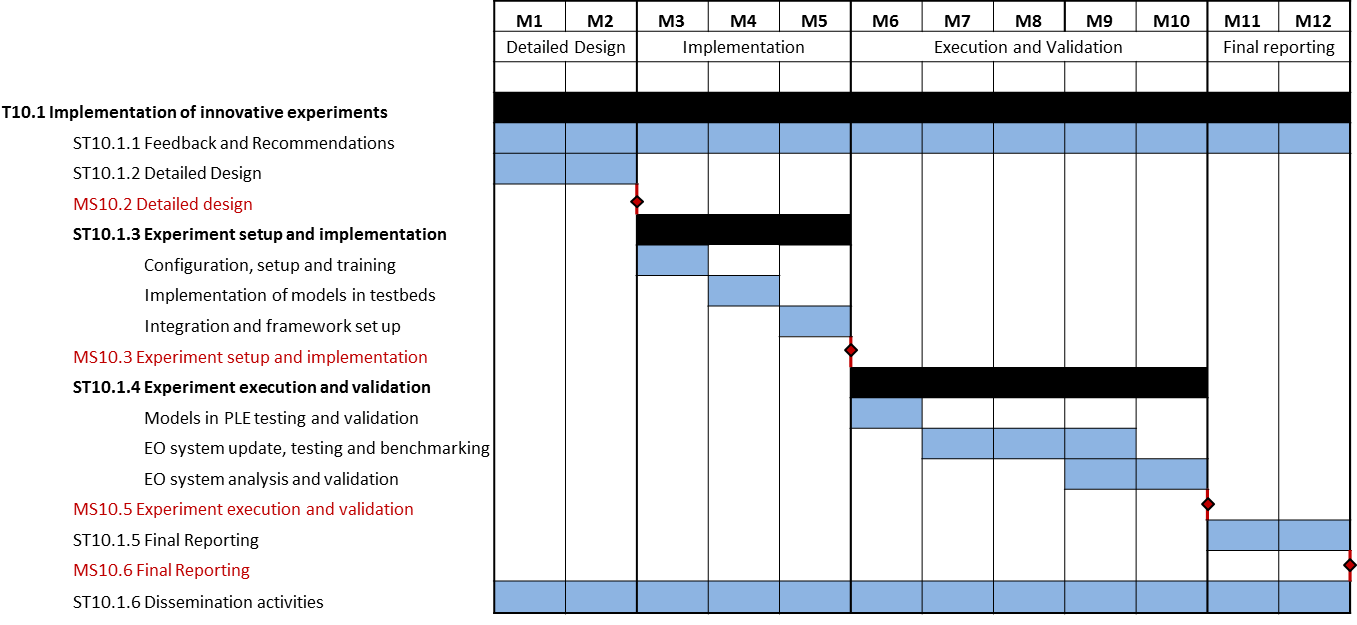
\includegraphics[width=6.31207in,height=2.90748in]{out-img8.png} 

{\centering\bfseries
Figure\ 4\ Experiment Schedule
\par}


\bigskip

The experiment has been divided into four stages by following the
Fed4FIRE timeline:


\bigskip

\liststyleLFOxli
\begin{itemize}
\item \textbf{Stage 1: Detailed Design}\ involves the detailed design of
the experiment.
\end{itemize}

\bigskip

\liststyleLFOxli
\begin{itemize}
\item \textbf{Stage 2:}\ \textbf{Experiment Setup and
Implementation\ }is devoted to the configuration and set up of the
testbeds,\ adaptation of the software\ modules\ and models for their
implementation in Virtual\ Wall, PlanetLab Europe\ and BonFIRE.\ 
\end{itemize}

\bigskip

\liststyleLFOxli
\begin{itemize}
\item \textbf{Stage 3:}\ \textbf{Experiment execution and
validation}\ includes the execution of the tests, their validation and
analysis.\ 
\end{itemize}

\bigskip

\liststyleLFOxli
\begin{itemize}
\item \textbf{Stage 4:}\ \textbf{Final reporting\ }involves the final
reporting of the experiment.\ 
\end{itemize}

\bigskip


\bigskip

\section[Ethical Issues]{Ethical Issues}
\hypertarget{Toc378868693}{}
\bigskip

The GEO-Cloud experiment will follow the ethical guidelines already
defined by the Fed4FIRE project. In addition, the experiment does\ not
raise any sensitive ethical questions nor does it include any critical
ethical aspects.\ The documentation generated will be objective and
transparent and third parties will be disclosed to access the data
collected during the experiment.


\bigskip

Fed4FIRE partners are invited to ethically review and monitor the
experiment. Adequate actuations will be carried out for their
suggestions and concerns.

\section[Conclusions]{Conclusions}
\hypertarget{Toc378868694}{}
\bigskip

In this deliverable we presented the Problem Statement of the GEO-Cloud
experiment and the Requirements defined to succeed on its
implementation and execution\ in Fed4FIRE.


\bigskip

In the\ first sections\ of the document we exposed the importance of the
Earth Observation field in European Research and the problems that
currently presents.\ Among such problems we find the lack of
flexibility and scalability of traditional data centers,
characteristics that are necessary to provide on demand services.\ The
GEO-Cloud experiment uses the future internet technologies to find
viable solutions to such problems.


\bigskip

The scenario is that of a constellation of Earth Observation satellites
that record images of the whole world in a daily basis to provide added
value services such as crisis management or emergencies.\ Such a
scenario is implemented in Fed4FIRE to emulate a real system using
future internet technology and measure its response and performance
when provided on demand services.\ 


\bigskip

For the implementation of the experiment three Fed4FIRE testbeds will be
used: PlanetLab Europe, Virtual Wall and BonFIRE.\ The schedule for the
GEO-Cloud implementation and execution is presented in\ Section 5.


\bigskip


\bigskip


\bigskip


\bigskip

\section{Bibliography}

\bigskip

Armbrust, M. (2010). A view of cloud computing.\ \textit{Communications
of the ACM, Vol. 53, N4}.

Deren, L. (2007). Remote sensing can help monitoring and predication
antural disasters, Vol.25, N6.

Simchi-Levi, D., Kaminsky, P., \& Simchi-Levy, E.
(1999).\ \textit{Designing and managing the supply chain: concepts,
strategies and cases.}\ McGraw-Hill.


\bigskip


\bigskip


\bigskip
\end{document}
